\documentclass[10pt]{article}
\usepackage[a4paper,margin=22mm]{geometry}
\usepackage[T1]{fontenc}
\usepackage{mathptmx}
\usepackage{amsmath,amssymb}
\usepackage{graphicx}
\usepackage{booktabs}
\usepackage{url}
\usepackage[font=small,labelfont=bf,labelsep=period]{caption}
\usepackage{titlesec}
\titleformat{\section}{\normalfont\large\bfseries}{\thesection.}{0.5em}{}
\titleformat{\subsection}{\normalfont\normalsize\bfseries}{\thesubsection}{0.5em}{}
\renewcommand{\thesection}{S\arabic{section}}
\renewcommand{\thetable}{S\arabic{table}}
\renewcommand{\thefigure}{S\arabic{figure}}
\setlength{\parskip}{3pt}
\newcommand{\sq}{\,\text{s}}

\begin{document}

\begin{center}
{\Large\bfseries Supplementary Material}\\[4pt]
{\large Watermark-Based Online EV--Charger Matching from Delayed Slot-Unlabeled Telemetry}\\[6pt]
Jiseok Yang and Daisuke Kodaira\\
University of Tsukuba, Japan\\[2pt]
{\small IEEE Access, manuscript Access-2026-34370 (revised version)}
\end{center}

\noindent This document collects the detailed results that the main manuscript summarizes in one or two sentences. Section, equation, figure, and table numbers without the prefix ``S'' refer to the main manuscript. Every value is taken from the same simulation evidence as the manuscript and is regenerated by the reproduction driver of the public repository cited as reference [42] of the manuscript, on the seeds stated in each caption. ``Global'' denotes the prior static correlation--DTW cost of [10], transferred unchanged into the online runtime.

\section{Dense-Sampling Diagnostic (Section VI-B)}

Every waveform cost is less accurate at 5\sq{} EV sampling than at 30\sq{} (Fig.~4). Table~\ref{tab:sampling} reports the diagnostics that locate the cause.

\emph{Not the number of points.} For every $\Delta t_{\text{EV}}$ the matching cost is evaluated on the same fixed 73-point, 5\sq{} decision grid ($W/5\sq + 1$ points from the EV-side start estimate), onto which the EV series is forward-filled. The denser setting therefore carries more independent measurements (independent samples at 5\sq, six copies of one sample at 30\sq) and is nevertheless the less accurate one.

\emph{Not a signal-to-noise effect.} With the per-sample noise removed (row ii) the trend persists at every $\Delta t_{\text{EV}}$; this control also moves the $\geq 1$\,A start detector that anchors the decision grid ($p_{90}$ latency 445 against 416\sq). Averaging the dense samples onto 30\sq{} blocks (row iii) lowers accuracy rather than recovering the 30\sq{} value.

\emph{Not the normalization.} The refined cost divides by the number of compared prefix points (73 at the full prefix, 44 at the 60\,\% stage), which does not depend on $\Delta t_{\text{EV}}$; path-length normalization is used only by the Global matcher. At the 60\,\% stage the step signature of Eq.~(8) sees only the 44-point prefix: the fourth step is only partly covered, and the fifth and sixth steps, which lie beyond the prefix, take the median of the whole prefix on both planes. The $\sigma_i$ scaling of Eq.~(14) is a per-decision spread across candidates and is absent from the Greedy matcher, which shows the same trend; the posterior stages of Eq.~(13) consume the same refined cost with weights that do not depend on $\Delta t_{\text{EV}}$.

\emph{The banded DTW term.} Partitioning Eq.~(7) (row iv), the DTW-only Greedy cost gains $+9.4 \pm 0.6$\,pt from 5 to 30\sq, whereas the step-signature-only cost does not ($+0.9 \pm 0.9$\,pt, not detectable at this sample size); the Global matcher, whose waveform score is correlation times DTW, shows the same dependence.

\emph{The cause: time alignment.} Each EV-side sample reads the slot current 5--25\sq{} ahead of its timestamp (Section V-A), a per-session lead. At 30\sq{} sampling a change in the slot current enters the held EV series at the first sampling instant whose read time reaches it, anywhere within the 30\sq{} period, so the lead is spread over about $-25$ to $+25$\sq{} and centered near zero. At 5\sq{} sampling that quantization is at most 5\sq, so the EV series leads the charger grid by up to five 5\sq{} samples---beyond the $\pm 15$\sq{} (three-sample) Sakoe--Chiba band of Eq.~(7) in about half of the sessions---and the correlation term of the Global cost, which pairs the two series at equal timestamps, is misaligned by the same lead (its DTW term is unbanded). In the alignment control (row v), with the per-session offset fixed at 5\sq{} (one charger sample) and every other setting unchanged, every waveform cost recovers to 0.999 or above at 5\sq{} sampling ($+0.050$ to $+0.064$ against the modeled offset, every paired 95\,\% CI excluding zero; the DTW-only cost $+0.097$), and the Posterior--Global difference vanishes ($-0.0002$; 95\,\% CI $-0.0006$ to $+0.0002$). Whether a wider band alone would recover the two banded costs was not tested, because the band is part of their calibrated cost; the remedy is a per-session calibration of the EV-side timestamp offset. The Posterior--Greedy difference is $+0.015 \pm 0.004$ at 5\sq, not detectable at this sample size at 15\sq, and $+0.011 \pm 0.003$ at 30\sq.

\begin{table}[h]
\centering
\caption{Dense-sampling diagnostic at the representative point ($EV = 500$, 50 slots, $d_{\max} = 10$\sq, $\Delta = 120$\sq; 20 paired repeats on the canonical seeds of each $\Delta t_{\text{EV}}$ cell; 95\,\% confidence intervals at most 0.008). (i) Manuscript front end (Section V-A sensing, forward-fill hold). (ii) EV sample-noise standard deviation set to 0\,A with gain, bias, extra sampling offset, and start-estimate jitter kept. (iii) The $\Delta t_{\text{EV}}$ samples averaged inside each 30\sq{} block before the 5\sq{} forward fill. (iv) Term partition of the Greedy cost, Eq.~(7): DTW term only / step-signature term only. (v) Alignment control: the per-session sensing offset fixed at 5\sq{} (one charger sample) with the Section V-A gain, bias, noise, and start-estimate jitter kept ($p_{90}$ latency 423\sq); run at 5\sq{} sampling only.}
\label{tab:sampling}
\small
\begin{tabular}{@{}lccc@{}}
\toprule
& \multicolumn{3}{c}{\textbf{EV sampling period} $\Delta t_{\text{EV}}$} \\
\cmidrule(lr){2-4}
\textbf{Front end / cost} & \textbf{5\sq} & \textbf{15\sq} & \textbf{30\sq} \\
\midrule
(i) Manuscript front end, Greedy & 0.935 & 0.969 & 0.973 \\
(i) Manuscript front end, Posterior & 0.950 & 0.968 & 0.984 \\
(ii) Sample noise off, Greedy & 0.947 & 0.966 & 0.977 \\
(ii) Sample noise off, Posterior & 0.949 & 0.966 & 0.983 \\
(iii) 30\sq{} block mean, Greedy & 0.930 & 0.954 & -- \\
(iii) 30\sq{} block mean, Posterior & 0.944 & 0.960 & -- \\
(iv) Greedy term partition, DTW only & 0.903 & 0.977 & 0.996 \\
(iv) Greedy term partition, step only & 0.912 & 0.942 & 0.921 \\
(v) Offset fixed at 5\sq, Greedy & 0.999 & -- & -- \\
(v) Offset fixed at 5\sq, Posterior & 1.000 & -- & -- \\
(v) Offset fixed at 5\sq, Global & 1.000 & -- & -- \\
(v) Offset fixed at 5\sq, Greedy DTW only & 1.000 & -- & -- \\
\bottomrule
\end{tabular}
\end{table}

\section{Static-Limit Check (Section VI-A)}

Table~\ref{tab:static} runs the online runtime in the static regime of [10]: 300 sessions arriving at $t = 0$ on 300 slots, complete 360\sq{} waveforms, no cloud-ingestion delay or loss, all 300 slots as candidates, and the prior study's interval codebook with fixed slot binding (20 repeats; seeds and scenario hashes shared by all matchers). With the five sensing-distortion parameters set to zero (ST-ideal), the prior correlation--DTW cost and the Posterior matcher both identify every pair (1.000 in all 20 repeats), reproducing the $>99\,\%$ reported in [10]; the Greedy matcher, whose one-to-one selection is greedy rather than Hungarian, reaches 0.677. With the sensing layer of Section V-A switched on (ST-paper), the static limit falls to 0.952 for the prior cost and to 0.626 for the Posterior matcher (Greedy 0.581; paired Posterior--Global difference $-0.327 \pm 0.016$).

The prior study's 300 patterns are separated by level (minimum pairwise $\ell_1$ setpoint distance 1--4\,A per repeat, mean 3\,A); the per-session gain and bias draws remove that separation for the ampere-scale step-signature terms of the Greedy and Posterior costs, whereas the correlation term of the prior cost is invariant to them. The sensing layer also spreads the EV-side start estimates (start-estimate jitter, and the $\geq 1$\,A detector acting on biased readings), so the 300 decisions of ST-paper fall on several watermark ticks and each tick's one-to-one assignment covers only the sessions decided at it, whereas ST-ideal decides all 300 sessions at one tick; the two effects are not separated here. The online base cell differs from the ideal static cell not only in online operation (asynchronous arrivals, ingestion delay and loss, and time gating to about 28 candidates instead of 300) but also in the sensing layer and in the codebook, so the contrast does not isolate the cost of going online. What it does show is that the runtime reaches the prior figure with the prior cost (0.999 online against 1.000 in the ideal static cell) and that the Posterior matcher ends 1.6\,pt below its ideal static value (0.984 against 1.000), a difference that the contrast cannot apportion among those changes. Nor does the sensing-on static cell separate candidate count from the codebook: every session there competes with the 299 other patterns, whose closest pairs lie 1--4\,A apart (38--68 pairs per repeat within 8\,A), whereas only 13 of the 10\,000 decisions of the online base cell face a gated competitor within 10\,A.

\begin{table}[h]
\centering
\caption{Static-limit check: the online runtime in the static regime of [10]---300 sessions arriving at $t = 0$ on 300 slots (one session per slot, 10--60\,min), complete $W = 360$\sq{} waveforms, cloud ingestion disabled (zero delay, jitter, loss, and watermark bound), all 300 slots as candidates, the prior study's interval codebook with fixed slot binding; base seed 2187631072, 20 repeats, same scenarios for all matchers; mean $\pm$ 95\,\% Student-$t$ confidence interval. ST-ideal sets all five sensing-distortion parameters to zero; ST-paper uses the Section V-A defaults. The online row is the TABLE 6 point, for contrast.}
\label{tab:static}
\small
\begin{tabular}{@{}lccc@{}}
\toprule
\textbf{Cell} & \textbf{Greedy} & \textbf{Global (prior)} & \textbf{Posterior} \\
\midrule
ST-ideal (sensing off) & 0.677 $\pm$ 0.020 & 1.000 $\pm$ 0.000 & 1.000 $\pm$ 0.000 \\
ST-paper (Sec.~V-A sensing) & 0.581 $\pm$ 0.014 & 0.952 $\pm$ 0.006 & 0.626 $\pm$ 0.016 \\
Online, TABLE 6 point & 0.973 & 0.999 & 0.984 \\
\bottomrule
\end{tabular}
\end{table}

\section{Cost-Term Partition under Sensing Distortion (Sections VI-A and VI-C)}

The step-signature term of Eq.~(8) compares per-step medians in amperes, so the per-session gain and bias of the sensing layer enter it directly, whereas the z-normalized DTW term of Eq.~(7) and the correlation term of Eq.~(9) are invariant to an affine change of the EV-side scale. Table~\ref{tab:termpart} measures the consequence on the sensing axis of Fig.~5(c): with the step term removed, the banded DTW cost alone reaches 0.996 at base load and 0.995 / 0.992 at sensing $\times 4$ / $\times 8$, above every matcher as configured (Global 0.975 / 0.921), whereas the step term alone falls to 0.860 / 0.743; the Global matcher's robustness rests on its correlation term (0.747 / 0.535 without it, against 0.969 / 0.963 without DTW). The partition is a diagnosis, not a re-tuned method: the DTW-only variant is ranked on the evaluation slice, so adopting it would be tuning on that slice, and the frozen TABLE 2 costs are kept throughout.

\begin{table}[h]
\centering
\caption{Cost-term partition under sensing distortion at the representative point ($EV = 500$, 50 slots, TABLE 6 seeds, 20 paired repeats; 95\,\% confidence intervals at most 0.012). Greedy: Eq.~(7) with the step-signature term removed (DTW only) or the DTW term removed (step only). Global: Eq.~(9) with the correlation factor removed or the DTW factor removed. The multiplier scales the sensing-noise, gain, and bias standard deviations of Section V-A as in Fig.~5(c); the gain stays clipped to $[0.8, 1.2]$.}
\label{tab:termpart}
\small
\begin{tabular}{@{}l ccc ccc@{}}
\toprule
& \multicolumn{3}{c}{\textbf{Greedy, Eq.~(7)}} & \multicolumn{3}{c}{\textbf{Global, Eq.~(9)}} \\
\cmidrule(lr){2-4} \cmidrule(lr){5-7}
\textbf{Sensing} & Full & DTW only & Step only & Full & No corr. & No DTW \\
\midrule
$\times 1$ (base) & 0.973 & 0.996 & 0.921 & 0.999 & 0.972 & 0.970 \\
$\times 4$ & 0.941 & 0.995 & 0.860 & 0.975 & 0.747 & 0.969 \\
$\times 8$ & 0.869 & 0.992 & 0.743 & 0.921 & 0.535 & 0.963 \\
\bottomrule
\end{tabular}
\end{table}

\section{Hyperparameter Sensitivity of the Posterior Matcher (Section VI-B)}

Table~\ref{tab:hyper} varies the three Posterior hyperparameters one at a time around their TABLE 2 values on the evaluation repeats of the representative point (Posterior matcher only; no value was re-selected). All fifteen cells lie in 0.9815--0.9838, every one above the Greedy reference (0.973) and below the Global reference (0.999); $\eta_{\text{mix}}$ and $\beta_{\text{curr}}$ change the result by at most 0.0002, and $\gamma_{\text{prev}}$ by at most 0.0023 (0.9815 at 0.30; paired difference $-0.0023 \pm 0.0019$, detectable but below 0.3\,pt), with the frozen value 0.60 at the top of the grid.

\begin{table}[h]
\centering
\caption{Sensitivity of the Posterior matcher to its hyperparameters at the representative point (evaluation repeats 1--20, seeds identical to TABLE 6); one hyperparameter varied at a time with the other two at their TABLE 2 values (bold); 95\,\% confidence intervals are 0.003 in every cell; Greedy reference 0.973, Global reference 0.999. No value was re-selected.}
\label{tab:hyper}
\small
\begin{tabular}{@{}lccccc@{}}
\toprule
$\gamma_{\text{prev}}$ & 0.30 & 0.45 & \textbf{0.60} & 0.75 & 0.90 \\
Accuracy & 0.9815 & 0.9829 & \textbf{0.9838} & 0.9833 & 0.9830 \\
\midrule
$\eta_{\text{mix}}$ & 0.15 & 0.25 & \textbf{0.35} & 0.50 & 0.70 \\
Accuracy & 0.9836 & 0.9838 & \textbf{0.9838} & 0.9838 & 0.9838 \\
\midrule
$\beta_{\text{curr}}$ & 0.50 & 0.75 & \textbf{1.00} & 1.50 & 2.00 \\
Accuracy & 0.9838 & 0.9838 & \textbf{0.9838} & 0.9838 & 0.9837 \\
\bottomrule
\end{tabular}
\end{table}

\section{Posterior Belief within One Decision (Section VI-C)}

Fig.~\ref{fig:posterior} records how the normalized beliefs of the top-1 and top-2 candidates of a representative session separate across the checkpoint updates of a single watermark decision: three checkpoints per stage, taken after the carry-over, time-prior, and current-likelihood factors of Eq.~(13). The checkpoint axis is not a runtime decision-tick sequence. The traced session reaches its full-window effective end 360\sq{} after its EV-side start estimate ($t_{\text{eff}} = \hat{t}_{\text{start}} + W$) and becomes mature 10\sq{} later ($t_{\text{wm}} = t_{\text{eff}} + d_{\max}$, Eq.~(2)). Success and failure cases alike are finalized through the ordinary watermark path. Beyond the second prefix, the posterior form contributes this normalized per-candidate belief, whose gap separates the near-ties among the residual errors: over all 162 errors of TABLE 8 the chosen and the true slot average 0.340 and 0.247, and within the near-ties (43\,\% of the errors, gap below 0.05) 0.275 and 0.252.

\begin{figure}[h]
\centering
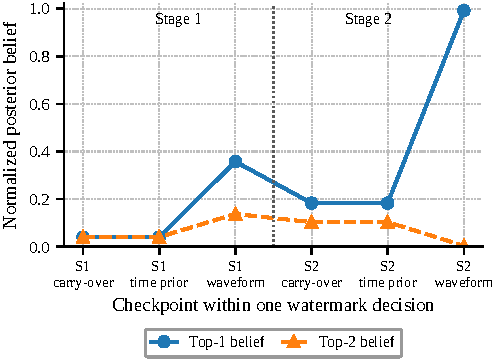
\includegraphics[width=0.62\textwidth]{figure5_posterior_diagnostic.pdf}
\caption{Normalized posterior belief of the top-1 and top-2 candidates of a representative session at the representative operating point ($EV = 500$) at the six checkpoints of a single watermark decision: after the carry-over, the time prior, and the waveform likelihood of Stage~1 (S1) and of Stage~2 (S2). Each checkpoint is the renormalized partial combination of Eq.~(13); the checkpoints lie inside one decision and are not finalization times or runtime ticks.}
\label{fig:posterior}
\end{figure}

\section{Additional Details for Sections VI and VII}

\textbf{Response heterogeneity (Fig.~6).} Realized draws over the 20 repeats: first-step lag 2--30\sq{} (mean 16.1\sq), rise rate 1.00--10.00\,A/s (mean 5.50\,A/s). The fitted rise rate (0.41--1.16\,A/s over the setpoint changes in use) lies at the slow edge of the drawn range, so the heterogeneous fleet responds faster than the calibration pair, whereas the drawn first-step lags bracket the fitted 15\sq{} on both sides. The paired 95\,\% CIs of the Posterior matcher's loss are $\pm 0.4$ / $0.5$ / $0.3$\,pt at 100 / 300 / 500 sessions (excluding zero at 300 and 500); the Global matcher changes by $-0.02 \pm 0.06$\,pt. The gap between the prior cost and the Posterior matcher at 500 sessions widens from 1.6 to 3.4\,pt.

\textbf{Command-codebook separation (Fig.~7).} Each arriving session receives the free pattern with the largest minimum distance to the patterns of the active sessions; the distance is the Euclidean distance between the z-normalized six-step patterns plus three small terms that compare level, step change, and mean level. The per-repeat minimum pairwise $\ell_1$ setpoint distances average 8.0, 4.5, 1.7, and 2.0\,A for the 6--30, 6--20, 8--16, and 8--12\,A bands. The accuracies per band (Global / Posterior / Greedy; 20 paired repeats, 95\,\% confidence intervals at most 0.006) are 0.999 / 0.984 / 0.973 at 6--30\,A, 0.996 / 0.974 / 0.968 at 6--20\,A, 0.981 / 0.948 / 0.936 at 8--16\,A, and 0.923 / 0.895 / 0.881 at 8--12\,A; the design rule of Section VI-B rests on the 8--16\,A band. Inside the base-load runs, the conditional error rate of the Posterior matcher, binned by the $\ell_1$ distance between the true pattern and its nearest pattern in the gated candidate set, is 7.7\,\% ($\leq 10$\,A; 13 decisions), 1.8\,\% (11--20\,A), 1.5\,\% (21--30\,A), 0.6\,\% (31--40\,A), and 0\,\% ($> 40$\,A), against 0.07\,\% in the two populated bins for the Global matcher; 40\,\% of the decisions have a competing candidate within 20\,A. Over all 162 errors of the Posterior matcher, the $\ell_1$ distance between the true and the chosen pattern has a median of 30\,A (minimum 13\,A).

\textbf{Saturation (TABLE 7).} Paired differences on admitted sessions: Posterior--Global $-0.039 \pm 0.004$ (S-A) and $-0.015 \pm 0.005$ (S-B); Posterior--Greedy $+0.012 \pm 0.003$ and $+0.003 \pm 0.003$. With fewer slots (S-B) the candidate sets shrink to at most 15 and the Greedy matcher gains (0.973 $\rightarrow$ 0.981).

\textbf{Latency decomposition (Section VI-A).} The start-estimate offset is the first 1\sq{} EV reading (rounded up to whole amperes) at or above 1\,A plus the $\pm 20$\sq{} start-estimate jitter. Because readings are rounded up, a session whose sensor reads a small positive value at 0\,A already reports 1\,A during the 0\,A first step, so for many sessions the detector fires within seconds of the arrival. The simulator keeps the estimate within $[t_{\text{arr}} - \Delta t_{\text{EV}},\, t_{\text{arr}} + W/2]$; with the Section V-A defaults this bound is not reached at $\Delta t_{\text{EV}} = 30$\sq{}, and it can bind at 5 and 15\sq{} sampling and in the strongest sensing cells. When the start estimate follows the arrival, the end of the decision grid lies past $t_{\text{arr}} + W$, mostly in the 0\,A first step of the re-issued pattern, on both planes (the EV plane holds its reading at $t_{\text{arr}} + W$, and the simulated charger current restarts from 0\,A without the 4\,A/s fall ramp). The reported 416\sq{} is the mean over the 20 repeats of the per-repeat 90th percentile, which the decomposition reproduces repeat by repeat.

\textbf{Operational side-effects (Section VII-D).} For a modulated time $T$ the charge not delivered is at most $T$ times the operator's limit (every setpoint at 0\,A) and, for a given codebook, $T$ times the difference between the limit and the pattern's mean setpoint. $T$ is at most 464\sq{} over the 10\,000 traced decisions. For the 6--30\,A codebook the mean setpoint over the 360\sq{} pattern is $\approx 15$\,A (including the 0\,A first step); assuming that mean over the whole of $T$, a constant 30\,A limit withholds $\approx 1.7$\,A$\cdot$h per phase at $T = 416$\sq, i.e., $\approx 0.35$--$0.40$\,kWh at 200--230\,V single-phase, about 1\,\% of a 40\,kWh battery (three times that on a three-phase unit). The upper bound at the same $T$ is 3.5\,A$\cdot$h per phase, $\approx 0.8$\,kWh at 230\,V, about 2\,\%. The setpoint changes are at most 30\,A per port (from the 0\,A first step to the largest setpoint; at most 24\,A between modulated steps) at 60\sq{} intervals. Because sessions arrive asynchronously, the windows of different ports are in general not synchronized; coincident window starts could be avoided by a site controller staggering the modulated windows.

\textbf{Duplicate claims (Section VII-E).} Among the 10\,000 traced decisions of TABLE 8, 198 pairs of sessions are finalized to the same slot while the earlier session is still connected (8 pairs for the Global matcher, which makes 7 errors), none of them decided in the same batch, and every pair contains a misidentified session---159 of the Posterior matcher's 162 errors appear in one. The count therefore tracks the error rate rather than adding to it.

\end{document}
